\documentclass[11pt,french]{report}
  \usepackage{babel} %%french
  \usepackage{amsmath,amsfonts,amssymb} %%maths
  \usepackage[utf8]{inputenc}   % LaTeX
  \usepackage[T1]{fontenc}      % LaTeX
  \usepackage[dvipsnames,table,xcdraw]{xcolor}
  %% Background code chunk
  \usepackage{listings}
  \usepackage{color}
 
  \definecolor{codegreen}{rgb}{0,0.6,0}
  \definecolor{codegray}{rgb}{0.5,0.5,0.5}
  \definecolor{codepurple}{rgb}{0.58,0,0.82}
  \definecolor{backcolour}{rgb}{0.95,0.95,0.92}
  
  %% image
  \usepackage{graphicx}
  	\graphicspath{{./fig/}} %fig path
  %%profondeur de la numérotation du TOC
  \setcounter{secnumdepth}{3} 
  %%lien hypertex
  \usepackage[colorlinks, allcolors=blue]{hyperref} 
  %% package pour modifier les chapitres #2
  \usepackage{titlesec}
  %% for number separation
  \usepackage[autolanguage]{numprint}
  %% for tikz picture
  \usepackage{tikz}
  %% for licence
  \usepackage{tabularx}
  \usepackage{multirow}
  %% no indent
  \setlength{\parindent}{0pt}
  \frenchbsetup{StandardItemLabels=true} % pour obtenir des puces par défaut dans les listes à puces A.B.
  %% for moreInfo    
  \usepackage{fontawesome} %%also cool logo
  \usepackage[framemethod=TikZ]{mdframed}
  %% set lenght figure
  \setlength{\abovecaptionskip}{5pt}
  %%abstract
  \usepackage{epigraph}
  %% background code chunk listing
  \lstset{
	language=R}
  \lstdefinestyle{mystyle}{
    backgroundcolor=\color{backcolour},   
    commentstyle=\color{codegreen},
    keywordstyle=\color{magenta},
    numberstyle=\tiny\color{codegray},
    stringstyle=\color{codepurple},
    basicstyle=\footnotesize,
    breakatwhitespace=false,         
    breaklines=true,                 
    captionpos=b,                    
    keepspaces=true,                 
    numbers=left,                    
    numbersep=5pt,                  
    showspaces=false,                
    showstringspaces=false,
    showtabs=false,                  
    tabsize=2
}

\lstset{style=mystyle}

%%maccro tikz bloc
\tikzset{
  block/.style = {draw, minimum width=5cm, minimum height=2.5cm, node distance=3cm},
  down/.style={yshift=-7em}
}

%macro position tikz
\newcommand{\tikzmark}[2]{\tikz[overlay, remember picture] \node[inner sep=0pt, outer sep=0pt, anchor=base] (#1) {#2};}


%maccro tilde
\def\utilde#1{\mathord{\vtop{\ialign{##\crcr
$\hfil\displaystyle{#1}\hfil$\crcr\noalign{\kern0.05pt\nointerlineskip}
$\hfil\tilde{}\hfil$\crcr\noalign{\kern0.05pt}}}}}

% Creation of environment to add additional informations
% Provided from Samuel Cabral Cruz
\mdfsetup{
	linewidth=2pt,
	nobreak=true,
	backgroundcolor=blue!10,
	roundcorner=10pt}	
\newenvironment{moreInfo}[1]
	{\begin{mdframed}
	\textcolor{darkgray}{\huge \raisebox{-3.5pt}{\faInfo} 
	\hspace{0.5cm} \large\bfseries #1}\\[5pt]
	\normalsize
	\makebox[0.1\textwidth][l]{}	
	\begin{minipage}{10cm}}
	{	\end{minipage}
	\end{mdframed}}

%maccro pour factoriel
\newcommand{\fact}[1]{#1\mathpunct{}!}

%% meta donnée document
\title{ACT 2003 \\ Notes de cours \\ Modèles linéaires en actuariat}
\author{\textbf{David Beauchemin}}
\date{\today}
\def\versionnumber{Automne 2017}

\usepackage{Sweave}
\begin{document}
\Sconcordance{concordance:notes_de_cours.tex:notes_de_cours.Rnw:%
1 107 1 1 0 137 1 1 22 1 2 22 1 1 9 1 2 3 1 1 6 1 2 20 1 1 14 1 2 29 1 %
1 9 1 2 42 1 1 23 1 2 194 1 1 16 1 2 13 1 1 17 1 2 129 1 1 3 2 0 1 3 1 %
0 1 3 1 0 1 3 1 0 1 3 4 0 1 2 209 1 1 15 1 2 4 1 1 5 4 0 4 1 1 3 1 0 2 %
2 3 0 1 2 13 1 1 19 1 2 1 1 1 4 7 0 1 4 7 0 1 2 218 1 1 3 2 0 1 3 1 0 1 %
1 3 0 1 2 290 1}


\makeatletter
  \begin{titlepage}
  \centering
      {\large \textbf{\textsc{UNIVERSITÉ LAVAL}}}\\
      \textsc{École d'actuariat}\\
    \vspace{2cm}
    \vspace{2cm}
      {\LARGE \textbf{\@title}} \\
    \vfill
       {\large \@author} \\
    \vspace{8cm}
        {\large\textbf{\versionnumber}}\\
    \vfill
  \end{titlepage}
\makeatother

%%%%license %%%%%
\small
{\copyright} {\the\year} David Beauchemin \\

\vspace{\baselineskip}


\includegraphics[height=7mm,keepaspectratio=true]{by-sa}\\%
Cette création est mise à disposition selon le contrat
\href{http://creativecommons.org/licenses/by-sa/4.0/deed.fr}{%
  Attribution-Partage dans les mêmes conditions 4.0 International} de
Creative Commons. En vertu de ce contrat, vous êtes libre de:
\begin{itemize}
\item \textbf{partager} --- reproduire, distribuer et communiquer
  l'{\oe}uvre;
\item \textbf{remixer} --- adapter l'{\oe}uvre;
\item utiliser cette {\oe}uvre à des fins commerciales.
\end{itemize}
Selon les conditions suivantes:

\begin{tabularx}{\linewidth}{@{}lX@{}}
  \raisebox{-9mm}[0mm][13mm]{%
    
\includegraphics[height=11mm,keepaspectratio=true]{by}} &
  \textbf{Attribution} --- Vous devez créditer l'{\oe}uvre, intégrer
  un lien vers le contrat et indiquer si des modifications ont été
  effectuées à l'{\oe}uvre. Vous devez indiquer ces informations par
  tous les moyens possibles, mais vous ne pouvez suggérer que
  l'offrant vous soutient ou soutient la façon dont vous avez utilisé
  son {\oe}uvre. \\
  \raisebox{-9mm}{
\includegraphics[height=11mm,keepaspectratio=true]{sa}}
  & \textbf{Partage dans les mêmes conditions} --- Dans le cas où vous
  modifiez, transformez ou créez à partir du matériel composant
  l'{\oe}uvre originale, vous devez diffuser l'{\oe}uvre modifiée dans
  les mêmes conditions, c'est-à-dire avec le même contrat avec lequel
  l'{\oe}uvre originale a été diffusée.
\end{tabularx}

\pagebreak
%%%%%%% Abstract %%%%%%%
\begin{abstract}
\begin{itshape}
abstrat
\end{itshape}
\end{abstract}

%%%%Remerciements %%%%%
%% remerciements

\subsubsection*{Remerciements}
% Samuel Cabral Cruz pour les infos bulles
% Frédérick pour la confiance
% École pour la confiance
% Thomas pour notes de cours en stats
blah blah

\tableofcontents

\newpage

%%%%%% Content %%%%%%%%

%%%%%%% Chapitre 1 %%%%%%%%
\chapter{Introduction}
L'établissement de prévisions joue un rôle central dans notre vie de tous les jours (prévisions météorologique, horoscope, etc.), et plus particulièrement dans celle des actuaires.

\subsection*{Objectifs de la régression}
Régulièrement en actuariat, on se questionne sur les effets de différentes variables sur d'autres. Par exemple,
\begin{itemize}
\item Quel est l'effet de l'âge sur la fréquence des sinistres automobiles ?
\item Quel est l'effet du sexe sur la mortalité ?
\end{itemize}

On cherche à étuider et déterminer les relations entre des variables mesurables à partir de données.

\subsection*{Deux grandes classes de variables mesurables :}
\begin{itemize}
\item Qualitatives : basées sur des opinions et/ou des intuitions.
\item Quantitatives : basées sur des observations, un modèle et des arguments mathématiques.
\end{itemize}

\subsection*{Deux \textit{grandes étapes} pour établir des prévisions quantitatives}
\begin{enumerate}
\item Bâtir le modèle et estimer les paramètres:
\begin{itemize}
\item[ex:] $F = M \times a$ Qui représente un modèle déterministe
\item[ex:] $Y =3 \times X + 6 + \epsilon_t \text{ ;où} \epsilon_t \sim N(0, 10)$ Qui représente un modèle probabiliste 
\end{itemize}
\item Calculer les prévisions à partir du modèle.
\end{enumerate}

\bigskip
Dans le cadre du cours, seulement les modèles probabilistes linéaires seront étudiez. 

%%%%%%%%%%%%%%% Chapitre 2 %%%%%%%%%%%%%%%%%%%%%%%%%%%%%
\chapter{Régression linéaire simple}

\section{Introduction}

De façon générale, en régression, nous avons :

\begin{tabularx}{\linewidth}{c|X|c}
\hline
Y & Variable dépendante, ou de réponse & Output \\
$X_1, X_2, ..., X_n$ & Soit n variables indépendantes ou explicatives, ou exogènes\footnote{Les variables $X_i$ sont indépendante par rapport à y, mais pas nécessairement entre elles.} & Input \\
$\beta_0, \beta_1, ... \beta_n$ & Les paramètres à estimer & \\
\hline
\end{tabularx}

\bigskip
\bigskip
Voici une illustration du concept de régression linéaire

%%% fig for the concept of regression operation
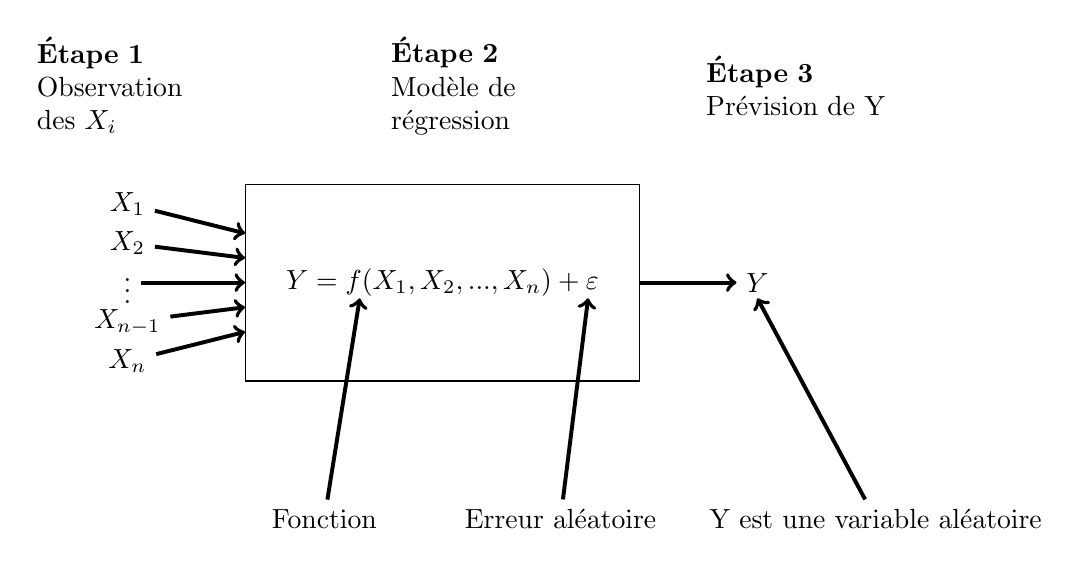
\begin{tikzpicture}
\node[block] (operator) at (4,1){$Y = f(X_1,X_2,...,X_n) + \varepsilon$};
\node[text width = 2.3cm] at (0,3.5) {\textbf{Étape 1} \\
									Observation des $X_i$};
\node[text width = 2.3cm] at (4.5,3.5) {\textbf{Étape 2} \\
									Modèle de régression};
\node[text width = 2.3cm] at (8.5,3.5) {\textbf{Étape 3} \\
									Prévision de Y};										
\node (a) at (0, 2) {$X_1$};
\draw[->, line width=0.5mm] ([right] a) --  (operator);
\node (b)at (0, 1.5) {$X_2$};
\draw[->, line width=0.5mm] ([right] b) --  (operator);
\node (c)at (0, 1) {$\vdots$};
\draw[->, line width=0.5mm] ([right] c) --  (operator);
\node (d)at (0, 0.5) {$X_{n-1}$};
\draw[->, line width=0.5mm] ([right] d) --  (operator);
\node (e)at (0, 0) {$X_{n}$};
\draw[->, line width=0.5mm] ([right] e) --  (operator);
\node (y)at (8, 1) {$Y$};
\draw[->, line width=0.5mm] (operator) -- ([left] y);
\node (F)at (2.5, -2) {Fonction};
\draw[->, line width=0.5mm] (F) --  (2.95, 0.8);
\node (E)at (5.5, -2) {Erreur aléatoire};
\draw[->, line width=0.5mm] (E) --  (5.85, 0.8);
\node (Y)at (9.5, -2) {Y est une variable aléatoire};
\draw[->, line width=0.5mm] (Y) --  (8, 0.8);
\end{tikzpicture}

\pagebreak

\subsection{Regression linéaire simple}

On cherche à prédire l'âge des passagers du Titanic selon le prix du billet à l'aide du modèle linéaire suivant,

\bigskip

%%% fig linéaire simple
\begin{center}
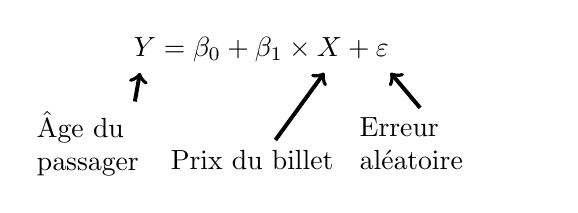
\begin{tikzpicture}[node distance=1.2cm]
\label{fig:linsimp}
\node (function) at (current page.center) {$Y  = \beta_0 + \beta_1 \times X + \varepsilon$};
\coordinate[below of=function] (c);
\node[text width = 2.3cm, left of=c, xshift=-0.5cm]  (Y) {Âge du passager};
\draw[->, line width=0.5mm] (Y) -- ([xshift=2mm, yshift=-3mm] function.west);
\node[text width = 2.3cm, below of=c, yshift=1cm] (X) {Prix du billet};
\draw[->, line width=0.5mm] (X) -- ([xshift=0.8cm, yshift=-3mm] function.center);
\node[text width = 2.3cm, right of=c, xshift=1.2cm] (E) {Erreur aléatoire};
\draw[->, line width=0.5mm] (E) -- ([xshift=-0.1cm, yshift=-3mm] function.east);
\end{tikzpicture}
\end{center}

%% Graphe modèle linéaire simple
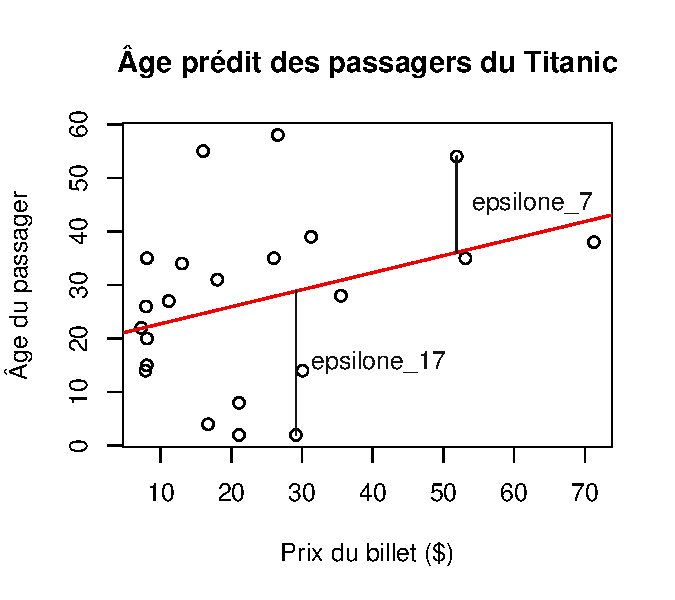
\includegraphics{notes_de_cours-001}

\subsection{Regression linéaire multiple}
On cherche à prédire l'âge des passagers du Titanic selon le prix du billet et son sexe à l'aide du modèle linéaire suivant,

\bigskip

%%% fig linéaire multiples
\begin{center}
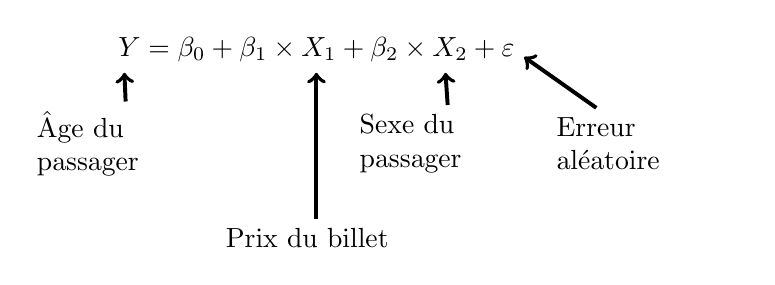
\begin{tikzpicture}[node distance=1.2cm]
\node (function) at (current page.center) {$Y  = \beta_0 + \beta_1 \times X_1 + \beta_2 \times X_2 + \varepsilon$};
\coordinate[below of=function] (c);
\node[text width = 2.3cm, left of=c, xshift=-1.2cm]  (Y) {Âge du passager};
\draw[->, line width=0.5mm] (Y) -- ([xshift=2mm, yshift=-3mm] function.west);
\node[text width = 2.3cm, below of=c, yshift=-0.0001cm] (X) {Prix du billet};
\draw[->, line width=0.5mm] (X) -- ([xshift=0cm, yshift=-3mm] function.center);
\node[text width = 2.3cm, right of=c, xshift=0.5cm] (X2) {Sexe du passager};
\draw[->, line width=0.5mm] (X2) -- ([xshift=-1cm, yshift=-3mm] function.east);
\node[text width = 2.3cm, right of=c, xshift=3cm] (E) {Erreur aléatoire};
\draw[->, line width=0.5mm] (E) -- ([ yshift=-1mm] function.east);
\end{tikzpicture}
\end{center}

%% fig 1 multilinear regression
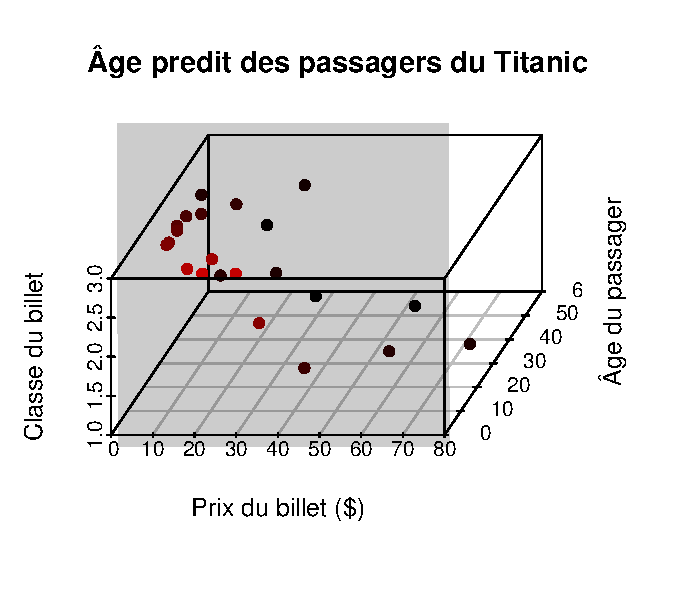
\includegraphics{notes_de_cours-002}


Voici la régression sous un autre angle, on voit la surface plane de régression.
%% fig 2
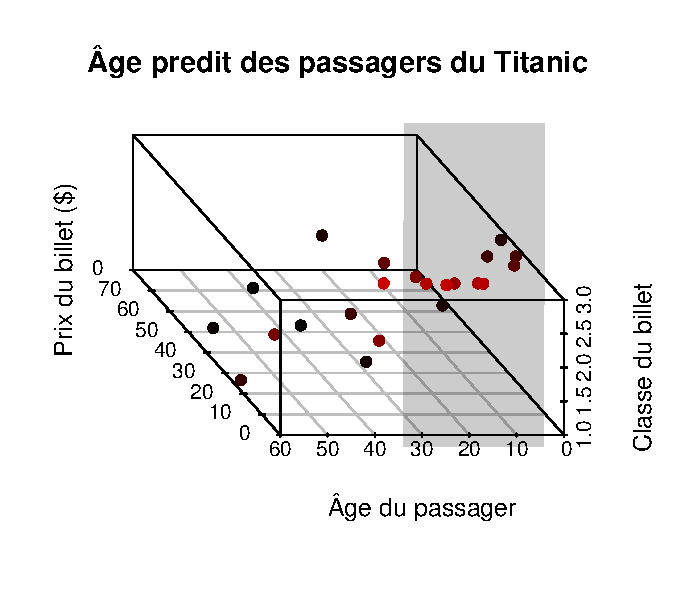
\includegraphics{notes_de_cours-003}



\subsection{Régression exponentielle}
On cherche à prédire la sévérité d'un sinistre automobile en fonction du temps à l'aide du modèle exponentielle suivant,

%%% fig exponentielle
\begin{center}
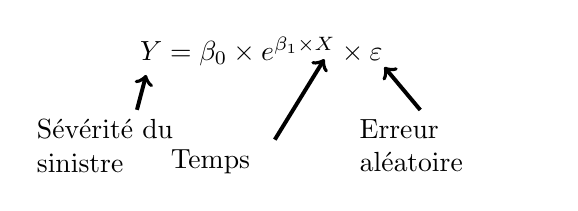
\begin{tikzpicture}[node distance=1.2cm]
\node (function) at (current page.center) {$Y  = \beta_0 \times  e^{\beta_1 \times X} \times \varepsilon$};
\coordinate[below of=function] (c);
\node[text width = 2.3cm, left of=c, xshift=-0.5cm]  (Y) {Sévérité du sinistre};
\draw[->, line width=0.5mm] (Y) -- ([xshift=2mm, yshift=-3mm] function.west);
\node[text width = 2.3cm, below of=c, yshift=1cm] (X) {Temps};
\draw[->, line width=0.5mm] (X) -- ([xshift=0.8cm, yshift=-1mm] function.center);
\node[text width = 2.3cm, right of=c, xshift=1.2cm] (E) {Erreur aléatoire};
\draw[->, line width=0.5mm] (E) -- ([xshift=-0.1cm, yshift=-2mm] function.east);
\end{tikzpicture}
\end{center}

%% Figure modèle exponentielle
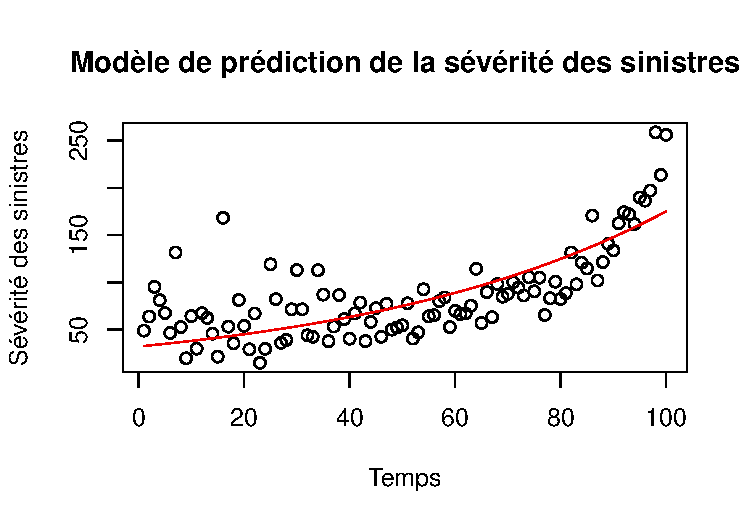
\includegraphics{notes_de_cours-004}


\subsubsection*{Note}
\label{note:exponentielle}
On remarque que la régression exponentielle est similaire à une régression linéaire simple.
\begin{align*}
\ln (Y) &= \ln (\beta_0) + \beta_1 \times X + \ln (\varepsilon) \\
Y^* &= \beta_0^* + \beta_1 \times X + \varepsilon^*\\
\end{align*}
Qu'on appel aussi une régression multiplicative ou log-linéaire.

\subsection{Régression quadratique}
On cherche à prédire la sévérité d'un sinistre automobile en fonction du temps et du temps au carré à l'aide du modèle quadratique suivant,

%%% fig quadratique
\begin{center}
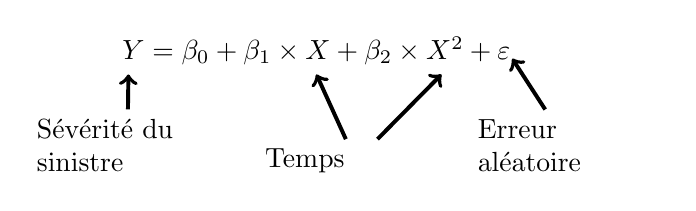
\begin{tikzpicture}[node distance=1.2cm]
\node (function) at (current page.center) {$Y  = \beta_0 + \beta_1 \times X + \beta_2 \times X^2 + \varepsilon$};
\coordinate[below of=function] (c);
\node[text width = 2.3cm, left of=c, xshift=-1.2cm]  (Y) {Sévérité du sinistre};
\draw[->, line width=0.5mm] (Y) -- ([xshift=2mm, yshift=-3mm] function.west);
\node[text width = 2.3cm, below of=c, yshift=1cm, xshift = 0.5cm] (X) {Temps};
\draw[->, line width=0.5mm] (X) -- ([xshift=0cm, yshift=-3mm] function.center);
\draw[->, line width=0.5mm] (X) -- ([xshift=-1cm, yshift=-3mm] function.east);
\node[text width = 2.3cm, right of=c, xshift=2cm] (E) {Erreur aléatoire};
\draw[->, line width=0.5mm] (E) -- ([yshift=-1mm, xshift = -1mm] function.east);
\end{tikzpicture}
\end{center}

%% Graphe modèle quadratique
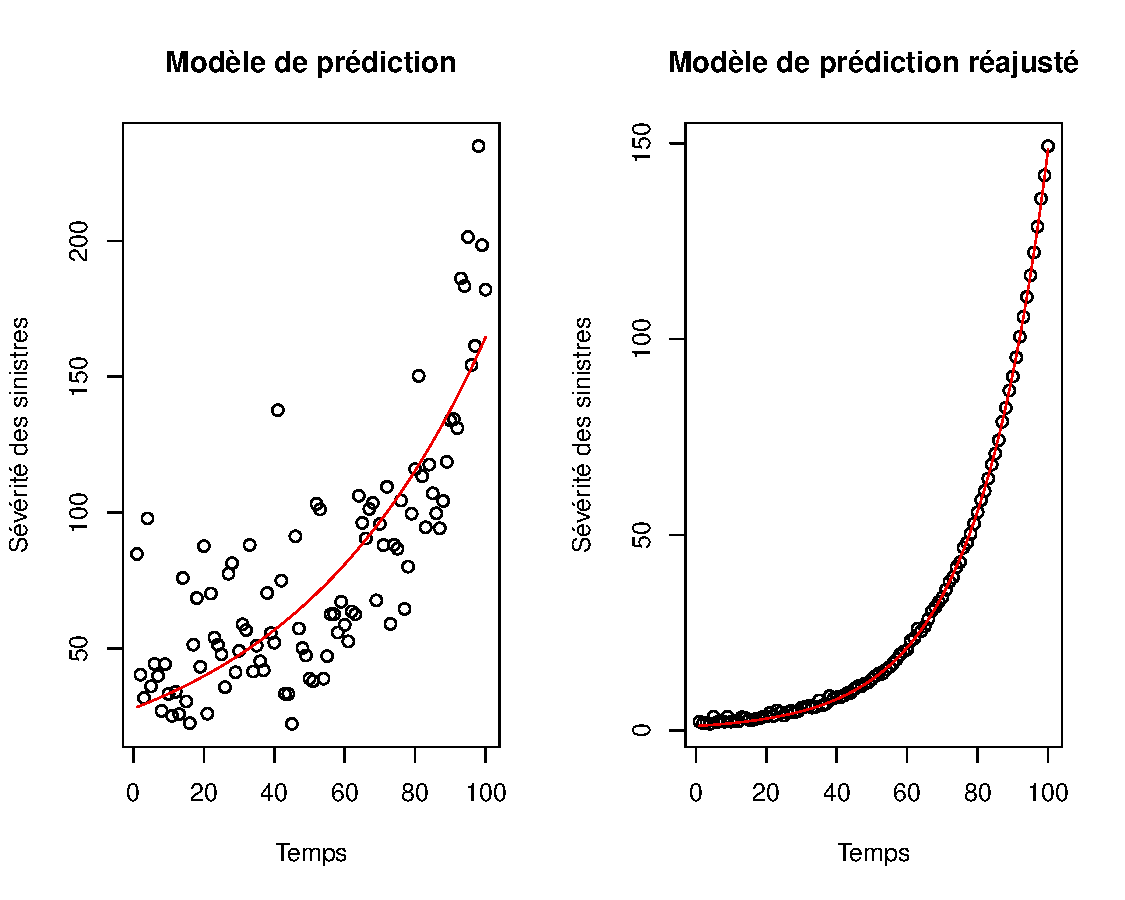
\includegraphics{notes_de_cours-005}

\subsubsection*{Note}
\label{note:quadratique}
On remarque que la régression quadratique est similaire à une régression linéaire multiple. En posant $X_1=X$ et $X_2 = X^2$
\begin{align*}
Y &= \beta_0 + \beta_1 \times X_1 + \beta_2 \times X_2 + \varepsilon\\
\end{align*}
Soit une régression linéaire multiple.

Dans le cadre du cours, seulement les modèles linéaires seront à l'étude car,

\begin{itemize}
\item Plus simples
\item Plusieurs modèles peuvent se ramener à un modèle linéaire simple ou multiple. (voir \ref{note:exponentielle} et \ref{note:quadratique})
\item Constituent souvent une très bonne approximation de la réalité qui peut être très complexe, tel que l'assurance.
\item Se généralisent faciment, tel que les \textit{Generalized Linear Models}.
\end{itemize}

Le principale problème de la modélisation linéaire est de trouver les différents paramètres $\beta_0, \beta_1, ..., \beta_n$ de tel sorte que
\begin{equation}
\varepsilon = Y - f(X_1,...,X_n; \beta_0, \beta_1,...,\beta_n)
\end{equation}
soit minimiser.

Il existe plusieurs méthode pour calcul l'erreur. Soit les erreurs suivants :
\begin{itemize}
\item Erreur totale
\item Erreur absolue
\item Erreur quadratique
\end{itemize}

Quel type d'erreur est suffisante pour déterminer $\varepsilon$ ?

\subsubsection{Erreur totale}
\begin{equation}
\sum_{t=1}^n \varepsilon_t = \sum_{t=1}^n \Big( Y_t - (\beta_0 + \beta_1\times X_t) \Big) 
\end{equation}
\begin{itemize}
\item Facile à mettre à 0
\item Pas fiable à cause de la mise à zéro
\end{itemize}

%% Graphe modèle quadratique
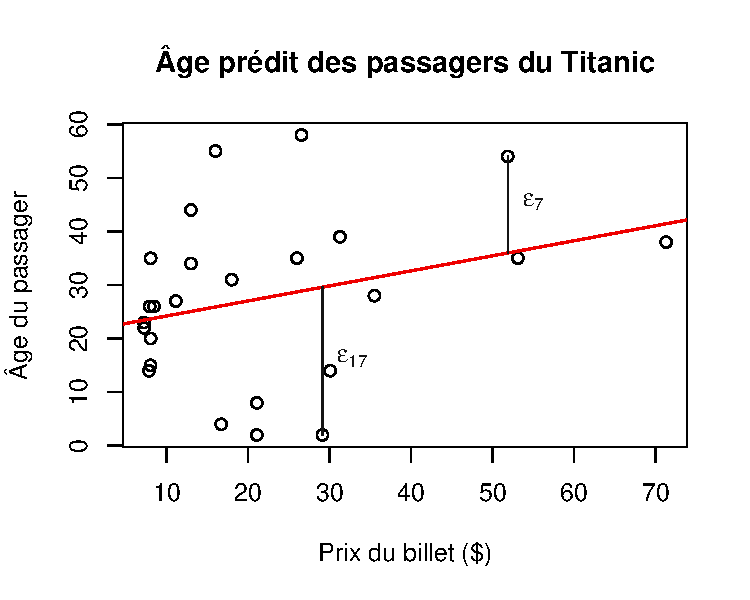
\includegraphics{notes_de_cours-006}


\subsubsection{Erreur absolue}
\begin{equation}
\sum_{t=1}^n |\varepsilon_t| = \sum_{t=1}^n \Big| Y_t - (\beta_0 + \beta_1\times X_t) \Big| 
\end{equation}
\begin{itemize}
\item Très robuste
\item Très compliqué mathématiquement, pour minimiser $\sum_{t=1}^n |\varepsilon_t|$ cela implique de dériver la fonction.
\end{itemize}

\subsubsection{Erreur quadratique}
\begin{equation}
\sum_{t=1}^n \varepsilon_t^2 = \sum_{t=1}^n \Big[ Y_t - (\beta_0 + \beta_1\times X_t) \Big]^2 
\end{equation}
\begin{itemize}
\item Mathématiquement plus simple que l'erreur quadratique.
\item Donne beaucoup de poids aux grandes erreurs
\end{itemize}

\bigskip
L'erreur quadratique semble donc l'option la plus simple dû à la facilité mathématique et ça fiabilité.

\section{Le modèle de régression linéaire simple}
Le modèle de régression linéaire simple tente d'expliquer le mieux possible la variable \href{https://fr.wikipedia.org/wiki/Variable_dépendante}{dépendante} \footnote{On appel parfois la variable dépendante une variable \href{https://fr.wikipedia.org/wiki/Endogène}{endogène}. Qui s'interpréte comme étant une variable qui est dû à une cause interne.}  Y à l'aide d'une variable \href{https://fr.wikipedia.org/wiki/Variable_indépendante}{indépendante}\footnote{On appel parfois les variables dépendantes des variables \href{https://fr.wikipedia.org/wiki/Exogène}{exogène}. Qui s'intrepréte comme étant extérieur à un système.} X . 

Si on dispose de n paires d'observations $(X_1, Y_1), (X_2, Y_2),...,(X_n, Y_n)$ alors, le modèle s'exprime  comme suit :
\begin{equation}
\label{eq:simple}
Y_i = \beta_0 + \beta_1\times X_i + \varepsilon_i \text{,  i = 1, ...,n.}
\end{equation}

Où $\beta_0$ est le paramètre associé à l'ordonnée à l'origine du modèle;
$\beta_1$ est le paramètre associé à la pende de la droite;
et $\varepsilon$ est le terme d'erreur.

\subsubsection*{Quelques remarques sur le modèle}
Dans l'équation \ref{eq:simple} du modèle, on remarque que 
\begin{itemize}
\item Les observations de $Y_i$ sont tiré d'une varaible aléatoire;
\item Les observations de $X_i$ sont considérées comme des valeurs connues et non aléatoires;
\item Les paramètres $\beta_0$ et $\beta_1$ sont inconnus au départ et doivent être estimer;
\item $\varepsilon_i$ sont des réalisations inconnues d'une variable aléatoire.
\end{itemize}

\subsubsection*{Exemple d'un modèle de régression}
\begin{align*}
X_t &: \text{nombre d'années de scolarité de l'actuaire} t \\
Y_t &: \text{Salaire de l'actuaire} t\\
\end{align*}

Comment résoudre le modèle pour prédire les salaires des actuaires en fonction du nombre d'années de scolarité ?

\bigskip
\textbf{Raisonnement:}
\begin{itemize}
\item Pour $X_t = 0$; on a $Y_t = \beta_0$. Autrement dit, le salaire avec un nombre d'année de scolarité est \emph{en moyenne} de $\beta_0$. Par exemple, $\beta_0$ serait le salaire moyen d'un stagiaire.
\item Par la suite, pour chaque année additionnelle de scolarité, le salaire augmente \emph{en moyenne }de $\beta_1$ unitées.
\end{itemize}
Ainsi, \emph{en moyenne} on a 
\begin{align*}
E[Y_t|X_t] &= \beta_0 + \beta_1\times X_t
\end{align*}

Habituellement, la relation n'est pas parfaitement exacte dans la réalité. On se retrouve ainsi avec une \emph{différence} dans notre variable exogène prédite. L'erreur est notée $\varepsilon_t$ et est tel que mentionnée plus tôt, assumée aléatoire.
\begin{align*}
\varepsilon_t &= Y_t - E[Y_t|X_t] \\
&= Y_t - (\beta_0 + \beta_1\times X_t)\\
\end{align*}

En réoganisant, on retrouve l'équation \ref{eq:simple}.
%%% fig linéaire simple 2
\begin{center}
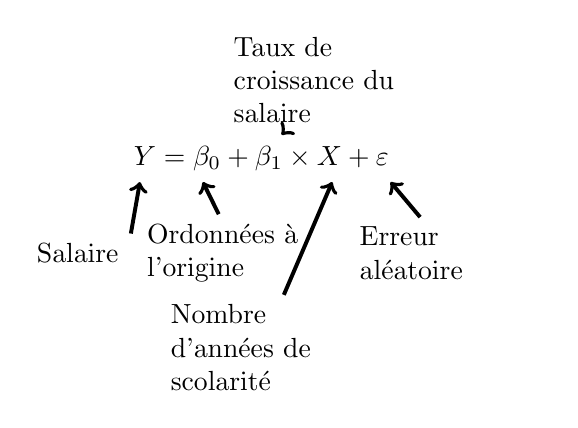
\begin{tikzpicture}[node distance=1.2cm]
\node (function) at (current page.center) {$Y  = \beta_0 + \beta_1 \times X + \varepsilon$};
\coordinate[below of=function] (c);
\node[text width = 2.3cm, left of=c, xshift=-0.5cm]  (Y) {Salaire};
\draw[->, line width=0.5mm] (Y) -- ([xshift=2mm, yshift=-3mm] function.west);
\node[text width = 2.3cm, left of=c, xshift=0.9cm]  (B) {Ordonnées à l'origine};
\draw[->, line width=0.5mm] (B) -- ([xshift=1cm, yshift=-3mm] function.west);
\node[text width = 2.5cm, above of=c, xshift=0.9cm, yshift=1cm]  (B2) {Taux de croissance du salaire};
\draw[->, line width=0.5mm] (B2) -- ([xshift=2cm, yshift=3mm] function.west);
\node[text width = 2.3cm, below of=c] (X) {Nombre d'années de scolarité};
\draw[->, line width=0.5mm] (X) -- ([xshift=0.9cm, yshift=-3mm] function.center);
\node[text width = 2.3cm, right of=c, xshift=1.2cm] (E) {Erreur aléatoire};
\draw[->, line width=0.5mm] (E) -- ([xshift=-0.1cm, yshift=-3mm] function.east);
\end{tikzpicture}
\end{center}

On doit maintenant trouver les paramètres $\beta_0$ et $\beta_1$ de manière à minimiser l'erreur $\varepsilon_t$.

Si $\varepsilon_t$ est minimal, cela veut dire que $Y_t \approx \beta_0 + \beta_1\times X_t$. Ce qui signifie que la droite de régression est une bonne approximation de $Y_t$.

\begin{moreInfo}{\emph{En résumé}}
	En résumé, on cherche à minimiser nos résidus en optimisant les paramètres $\beta_i$. 
\end{moreInfo}

\subsection{Coefficients de régression}
Les paramètres $\beta_0$ et $\beta_1$ sont déterminés en minimisant l'erreur quadratique à l'aide de la méthode des moindres carrées.

\begin{align*}
S(\beta_0, \beta_1) &= \sum_{t=1}^n \varepsilon_t^2 \\
&= \sum_{t=1}^n \big( Y_t - (\beta_0 + \beta_1\times X_t) \big)^2 \\
&= \sum_{t=1}^n \big( Y_t - \beta_0 - \beta_1\times X_t \big)^2 \\
\end{align*}

Où $S(\psi)$ peut être considéré comme une mesure de la \emph{distance} entre les données observées et le modèle théorique qui prédit ces données \footnote{Pour de plus ample information sur la méthode des moindres carrées et la fonction de \emph{distance}, la page \href{https://fr.wikipedia.org/wiki/Méthode_des_moindres_carrés}{Wikipédia} contient des bonnes explications sur le sujet.}.

\bigskip
Afin de minimiser la fonction $S(\beta_0, \beta_1)$ on dérive la fonction partiellement en fonction de chacun des paramètres.

\subsubsection*{Minimisation de $\beta_0$}
\begin{align*}
\frac{\partial S(\hat{\beta_0}, \hat{\beta_1})}{\partial \beta_0} &= 0 \\
\frac{\partial}{\partial \beta_0} \sum_{t=1}^n \big( Y_t - \hat{\beta_0} - \hat{\beta_1}\times X_t \big)^2 &= 0 \\
-2\sum_{t=1}^n \big( Y_t - \hat{\beta_0} - \hat{\beta_1} \times X_t \big) &= 0 \\
\end{align*}
\begin{equation}
\label{eq:minimisationbeta0}
\sum_{t=1}^n Y_t - n \times \hat{\beta_0} - \hat{\beta_1} \sum_{t=1}^n X_t = 0 \\
\end{equation}

\subsubsection*{Minimisation de $\beta_1$}
\begin{align*}
\frac{\partial S(\hat{\beta_0}, \hat{\beta_1})}{\partial \beta_1} &= 0 \\
\frac{\partial}{\partial \beta_1} \sum_{t=1}^n \big( Y_t - \hat{\beta_0} - \hat{\beta_1}\times X_t \big)^2 &= 0 \\
-2\sum_{t=1}^n \big( Y_t - \hat{\beta_0} - \hat{\beta_1} \times X_t \big) \times X_t &= 0 \\
\end{align*}
\begin{equation}
\label{eq:minimisationbeta1}
\sum_{t=1}^n Y_t \times X_t - \hat{\beta_0} \sum_{t=1}^n X_t - \hat{\beta_1} \sum_{t=1}^n X_t^2 = 0 \\
\end{equation}

À l'aide des équations \ref{eq:minimisationbeta0} et \ref{eq:minimisationbeta1}, on peut trouver les deux inconnus $\beta_0$ et $\beta_1$.

À partir de \ref{eq:minimisationbeta0} :

\begin{align*}
\sum_{t=1}^n Y_t - n \times \hat{\beta_0} - \hat{\beta_1} \sum_{t=1}^n X_t &= 0 \\
\sum_{t=1}^n Y_t - \hat{\beta_1} \sum_{t=1}^n X_t &=  n \times \hat{\beta_0} \\
\frac{\sum_{t=1}^n Y_t}{n} - \hat{\beta_1} \frac{\sum_{t=1}^n X_t}{n} &=  \hat{\beta_0} \\
\end{align*}

\begin{equation}
\label{eq:beta0}
\color{blue}
\boxed{\color{black}
\hat{\beta_0} = \overline{Y} - \hat{\beta_1} \overline{X}}
\end{equation}

Et à partir de \ref{eq:minimisationbeta1} :

\begin{align*}
\sum_{t=1}^n Y_t \times X_t - \hat{\beta_0} \sum_{t=1}^n X_t - \hat{\beta_1} \sum_{t=1}^n X_t^2 &= 0 \\
\sum_{t=1}^n Y_t \times X_t - \hat{\beta_0} \sum_{t=1}^n X_t &=  \hat{\beta_1} \sum_{t=1}^n X_t^2 \\
\end{align*}

\begin{equation}
\label{eq:beta}
\hat{\beta_1} =  \frac{\sum_{t=1}^n Y_t \times X_t - \hat{\beta_0} \sum_{t=1}^n X_t}{\sum_{t=1}^n X_t^2}
\end{equation}

On utilise l'équation \ref{eq:beta0} de $\hat{\beta_0}$ avec l'équation \ref{eq:beta} de $\hat{\beta_1}$, on développe l'équation résultante afin d'isoler $\hat{\beta_1}$.

\begin{align*}
\hat{\beta_1} &= \frac{\sum_{t=1}^n Y_t \times X_t - (\overline{Y} - \hat{\beta_1}\overline{X})\sum_{t=1}^n X_t}{\sum_{t=1}^n X_t^2} \\
&= \frac{\sum_{t=1}^n Y_t \times X_t - (\overline{Y} - \hat{\beta_1}\overline{X})\times n \overline{X}}{\sum_{t=1}^n X_t^2} \\
&= \frac{\sum_{t=1}^n Y_t X_t - n\overline{Y}\overline{X} + \hat{\beta_1}\times \overline{X}^2 \times n}{\sum_{t=1}^n X_t^2} \\
\end{align*}
En isolant $\hat{\beta}_1$, on obtient la définition suivante

\begin{equation}
\label{eq:beta1}
\color{blue}
\boxed{\color{black}
\hat{\beta_1} = \frac{\sum_{t=1}^n Y_t X_t - n\overline{Y}\overline{X}}{\sum_{t=1}^n X_t^2 - n\overline{X}^2}
}
\end{equation}

\subsubsection*{Remarques}

\begin{enumerate}
\item On note $\hat{\varepsilon}_t$ les résidus générés par le modèle estimé:
\begin{align*}
\hat{\varepsilon}_t &= Y_t - \hat{Y}_t \\
\hat{\varepsilon}_t &= Y_t - (\hat{\beta}_0 - \hat{\beta}_1 X_t) \text{; pour t = 1,2,...,n} \\
\end{align*}

Si on illustre graphiquement les résidus, il s'agit du segment le plus court entre la droite de régression et la donnée observée. 

\bigskip
Si on reprend le graphique de la section \ref{fig:linsimp}, on observe facilement les résidus sur cette représentation graphique :

%% Graphe modèle linéaire simple
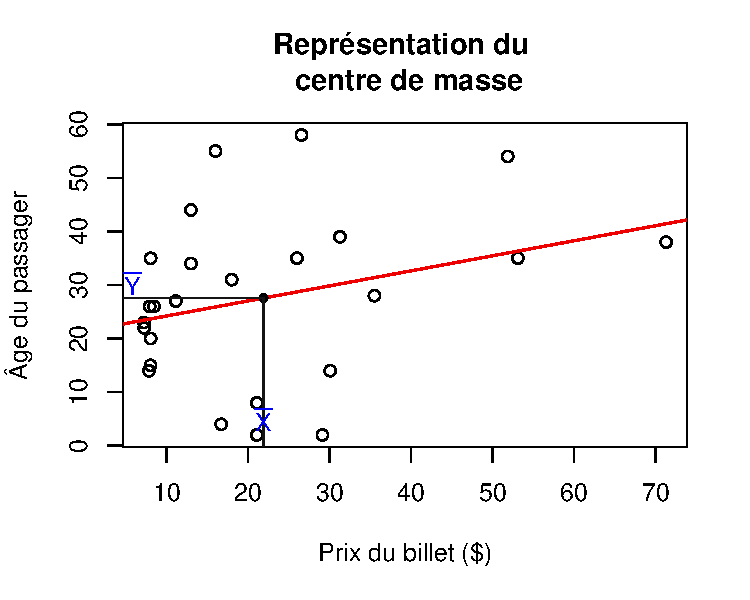
\includegraphics{notes_de_cours-007}

\item Le \emph{centre de gravité}\footnote{Qu'on appelle parfois centre de masse.} des données $(\overline{X}, \overline{Y})$ se trouve exactement sur la droite de régression.

On peut facilement effectuer cette preuve à partir de l'équation \ref{eq:beta0},
\begin{align*}
\hat{\beta_0} &= \overline{Y} - \hat{\beta_1} \overline{X} \\
\overline{Y} &=  \hat{\beta_0} + \hat{\beta_1} \overline{X} + 0 \\
\end{align*}
On note ainsi une absence de résidus pour le centre de masse.

\bigskip
Si on reprend (encore) le graphique de la section \ref{fig:linsimp}, on observe facilement le centre de masse sur le graphiqe. 

%% Graphe modèle Xbarre et Ybarre
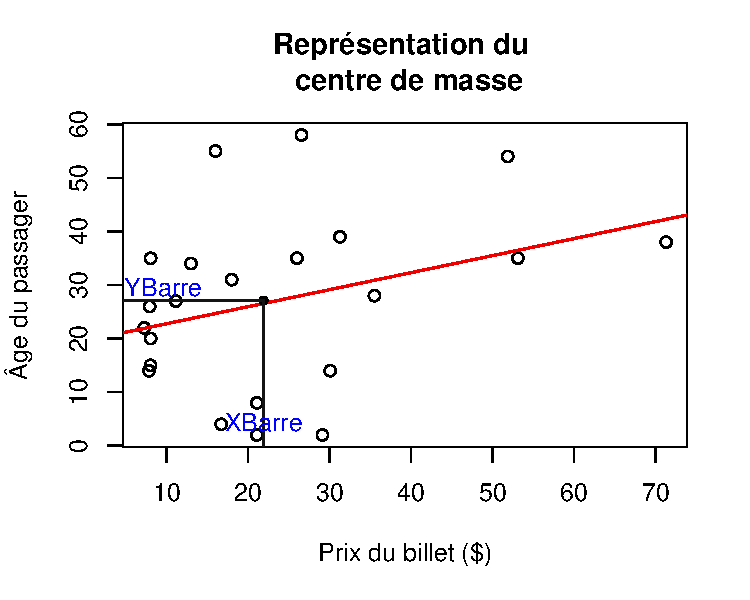
\includegraphics{notes_de_cours-008}

\item La somme des résidus de tout modèle de régression linéaire est nulle.
\begin{align*}
\sum_{t=1}^{n} \hat{\varepsilon}_t &= \sum_{t=1}^{n}\big( Y_t - (\hat{\beta}_0 + \hat{\beta}_1 X_t) \big) \\
&\overset{\ref{eq:beta0}}{=} \sum_{t=1}^{n}\big( Y_t - (\overline{Y} - \hat{\beta}_1 \overline{X}) \big) \\
&= \sum_{t=1}^{n} Y_t - \sum_{t=1}^{n}\overline{Y} + \hat{\beta}_1 \sum_{t=1}^{n}\overline{X} - \hat{\beta}_1\sum_{t=1}^{n}X_t \\
&= n \overline{Y} - n \overline{Y} + \hat{\beta}_1 + n \overline{X} - \hat{\beta}_1 + n \overline{X} \\
&= 0
\end{align*}
\end{enumerate}

\subsubsection*{Notation}
Afin de faciliter l'écriture, on intégre la notation suivante, $S_{xx}$ et  $S_{xy}$. Qui sont appelés respectivement la somme des carrées corrigée de $x$ et la somme des produits croisés corrigée de $x$ et de $y$.
Voici le développement pour $S_{xx}$,
\begin{align*}
S_{xx} &= \sum_{t=1}^n (X_t - \overline{X})^2 \\
&= \sum_{t=1}^n (X_t - \overline{X})^2 \\
&= \sum_{t=1}^n (X_t^2 - 2X_t\overline{X} + \overline{X}^2) \\
&= \sum_{t=1}^n X_t^2 - 2\overline{X}\sum_{t=1}^n X_t + n\overline{X}^2 \\
&= \sum_{t=1}^n X_t^2 - 2\overline{X}n\overline{X} + n\overline{X}^2 \\
&= \sum_{t=1}^n X_t^2 - n\overline{X}^2 \\
\end{align*}

On effectue le même type de développement pour $S_{xy}$, 
\begin{align*}
S_{xy} &= \sum_{t=1}^n (X_t - \overline{X}) (Y_t - \overline{Y}) \\
&\vdots \\
&= \sum_{t=1}^n X_tY_t - n\overline{X}\overline{Y}\\
\end{align*}

À l'aide des sommes de carrés corrigés, on peut réécrire la définition de $\hat{\beta}_1$

%% beta_1 en fonction de Sxx et Sxy
\begin{equation}
\label{eq:beta1SXY}
\color{blue}
\boxed{\color{black}
\hat{\beta_1} = \frac{S_{xy}}{S_{xy}}
}
\end{equation}

\bigskip
\subsubsection*{Exemple}
On poursuit avec un exemple pour assimiler l'information.

\bigskip
\begin{description}
\item[•] On dispose des cinq observations suivantes du couple $(X_t, Y_t)$ dans le tableau de gauche ainsi que les éléments calculer nécessaire pour trouver les paramètres dans le tableau de droite.
\end{description}

\begin{minipage}[t]{.4\linewidth}
\begin{tabular}{|c|c|c|}
\hline
t & $X_t$ & $Y_t$ \\
\hline
1 & 2 & 2 \\
2 & 3 & 5 \\
3 & 6 & 3 \\
4 & 9 & 6 \\
5 & 12 & 5 \\
\hline
Totaux : & 32 & 21 \\
\hline
\end{tabular}
\end{minipage}
\hfill
\begin{minipage}[t]{.4\linewidth}
\begin{tabular}{|c|c|c|}
\hline
t & $X_t^2$ & $X_tY_t$ \\
\hline
1 & 4 & 4 \\
2 & 9 & 15 \\
3 & 36 & 18 \\
4 & 81 & 54 \\
5 & 144 & 60 \\
\hline
Totaux : & 274 & 151 \\
\hline
\end{tabular}
\end{minipage}

\bigskip
%%calcul
À partir des définitions \ref{eq:beta0} et  \ref{eq:beta1}, on trouve facilement la valeur de $\hat{\beta}_0$ et de $\hat{\beta}_1$.

\begin{align*}
\hat{\beta_1} &= \frac{\sum_{t=1}^n Y_t X_t - n\overline{Y}\overline{X}}{\sum_{t=1}^n X_t^2 - n\overline{X}^2} \\
&= \frac{151 - (5)(\frac{21}{5})(\frac{32}{5})}{274 - (5)(\frac{32}{5})^2} \\
&= \frac{83}{346} \\
& \approx 0.2399 \\
\end{align*}

\begin{align*}
\hat{\beta_0} &= \overline{Y} - \hat{\beta_1} \overline{X} \\
&= \frac{21}{5} - (\frac{83}{346}) \times (\frac{32}{5}) \\
& \approx 2.6647
\end{align*}

On obtient ainsi le modèle de régression suivant :
\begin{align*}
Y_t &= 2.6647 + 0.2399X_t + \varepsilon_t
\end{align*}

\begin{center}
\begin{tabular}{|c|c|c|}
\hline
t & $Y_t = \hat{\beta}_0 + \hat{\beta}_1X_t$ & $\hat{\varepsilon}_t$ \\
\hline
1 & 3.1445 & -1.1445 \\
2 & 3.3844 & 1.6156 \\
3 & 4.1041 & -1.1041 \\
4 & 4.8238 & 1.1762 \\
5 & 5.5435 & -0.5435 \\
\hline
\end{tabular}
\end{center}

\begin{center}
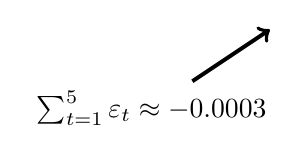
\begin{tikzpicture}[node distance=1.2cm]
\node (E) at (10,0) {$\sum_{t=1}^{5}\varepsilon_t \approx -0.0003$};
\draw[->, line width=0.5mm] (E) -- (11.5,1);
\end{tikzpicture}
\end{center}

\bigskip
\subsubsection*{Execution en R}
%% script R
\begin{lstlisting}[linerange=\\begin\{Sinput\}-\\end\{Sinput\},includerangemarker=false, caption = Code source en R pour l'exemple]
\begin{Schunk}
\begin{Sinput}
> # dataset
> x <- c(2,3,6,9,12); y <- c(2,5,3,6,5)
> # Estimations des parametres
> reg <- lm(y ~ x)
> # Resume de l'estimation
> summary(reg)
> # Valeurs de Yt
> fitted(reg)
> # Residus 
> residuals(reg)
\end{Sinput}
\end{Schunk}
\end{lstlisting}

\bigskip
%% info bull astuce calculatrice + reférence vers le guide
\begin{moreInfo}{\emph{Astuce calculatrice}}
	La calculatrice TI-30XS Multiview permet de créé un tableau de donnée et de sortir rapidement et facilement différentes informations sur une régression à partir des données. Tel que :
	\begin{itemize}
	\item $\overline{X}$ et $\overline{Y}$ ;
	\item $\sum_{t=1}^n X_t$, $\sum_{t=1}^n X_t^2$, $\sum_{t=1}^n Y_t$, $\sum_{t=1}^n Y_t^2$ et $\sum_{t=1}^n X_tY_t$ ;
	\item $\hat{\beta}_0$ et $\hat{\beta}_1$
	\end{itemize}
	Pour de plus ample information, consulter le \href{https://github.com/alpa12/guide_calculatrice}{guide} sur les calculatrices.
\end{moreInfo}
\bigskip

\subsection{Caractéristiques du terme d'erreur}
On rappel que l'équation du modèle de régression correspond à 

\begin{align*}
Y_t &= \beta_0 + \beta_1\times X_t + \varepsilon_t \text{ (\ref{eq:simple})}
\end{align*}
De plus, on sait qu'il s'agit des valeurs moyennes de $Y_t$ en sachat $X_t$, soit
\begin{align*}
Y_t = E[Y_t|X_t] + \varepsilon_t 
\end{align*}

On peut ainsi formuler les trois postulats \footnote{Le \href{https://fr.wikipedia.org/wiki/Postulat}{postulat} est un principe non démontré mais utilisé dans la construction d'une théorie mathématique. } suivants,
\begin{enumerate}
\item \label{post1} $E[\varepsilon_t] = 0$, par définition pour que $E[Y_t] = E[Y_t|X_t]$. Il s'agit de l'hypothèse de linéarité ou d'exogénéité de la variable explicative. On dit qu'elle est exogène si elle n'est pas corrélée au terme d'erreur.
\item \label{post2} $Var(\varepsilon_t) = \sigma^2$, la variance des termes d'erreurs est supposés constante. Il s'agit de l'hypothèse d'homoscédasticité.
\item \label{post3} $Cov(\varepsilon_t, \varepsilon_s) = 0$, pour $t \neq s$,il n'y a pas de corrélation entre les termes d'erreurs. Il s'agit de l'hypothèse d'indépendance des erreurs.
\end{enumerate}

\bigskip
%% info bull hypothèse implicite
\begin{moreInfo}{\emph{Quatrième postulat}}
	Les hypothèses de linéarité et d'homoscédasticité sont très intéressante, si on observe leurs définitions ensemble on remarque qu'il s'agit d'une distribution avec une espérance nulle et une variabilité supposé constante. Ce qui nous amène à une quatrième hypothése, les résidus sont distribués selon une loi normale.
	\begin{align*}
\hat{\varepsilon}_t|x_i \sim N(0, \sigma^2)
	\end{align*}
\end{moreInfo}
\bigskip

\subsection{Propriétés de l'estimateur des moindres carrées (EMC)}

\subsubsection{Estimateur sans biais}
On rappel qu'un estimateur est dit sans biais lorsque son espérance est égale à la valeur vrai du paramètre \footnote{note thomas}.

\begin{align*}
E[\hat{\beta}_1] &= E \Bigg[ \frac{\sum_{t=1}^n(X_t- \overline{X})(Y_t - \overline{Y})}{\sum_{t=1}^n(X_t - \overline{X})^2} \Bigg] \\
&= \frac{\sum_{t=1}^n(X_t- \overline{X})E[Y_t - \overline{Y}]}{\sum_{t=1}^n(X_t - \overline{X})^2} \\
&= \frac{\sum_{t=1}^n(X_t- \overline{X})(E[Y_t] - E[\overline{Y}])}{\sum_{t=1}^n(X_t - \overline{X})^2} \\
\end{align*}
De l'équation \ref{eq:simple}, et avec le postulat \ref{post1}, on sait que 

\begin{align*}
Y_t &= \beta_0 + \beta_1\times X_t + \varepsilon_t \\
E[Y_t] &= E[\beta_0 + \beta_1\times X_t] + E[\varepsilon_t] \\
&\overset{\ref{post1}}{=} \beta_0 + \beta_1\times X_t + 0 \\
\end{align*}
On applique le même raisonement pour l'espérance de $\overline{Y}$. 

\begin{align*}
E[\hat{\beta}_1] &= \frac{\sum_{t=1}^n(X_t- \overline{X})(E[Y_t] - E[\overline{Y}])}{\sum_{t=1}^n(X_t - \overline{X})^2} \\
&= \frac{\sum_{t=1}^n(X_t- \overline{X})(\beta_0 + \beta_1\times X_t - \beta_0 - \beta_1\overline{X_t})}{\sum_{t=1}^n(X_t - \overline{X})^2} \\
&= \frac{\sum_{t=1}^n(X_t- \overline{X})\beta_1 (X_t - \overline{X_t})}{\sum_{t=1}^n(X_t - \overline{X})^2} \\
&= \beta_1 \frac{\sum_{t=1}^n(X_t- \overline{X})^2}{\sum_{t=1}^n(X_t - \overline{X})^2} \\
E[\hat{\beta}_1] &= \beta_1
\end{align*}
\bigskip

Par conséquent,
\begin{align*}
E[\hat{\beta}_0] &= E[\overline{Y} - \hat{\beta}_1 \overline{X}] \\
&= E[\overline{Y}] - \overline{X} E[\hat{\beta}_1]  \\
&= \beta_0 + \beta_1\overline{X} - \overline{X}\beta_1 \\
E[\hat{\beta}_0]  &= \beta_0 \\
\end{align*}

On peut ainsi conclure que les deux estimateurs des paramètres sont sans biais.

\subsubsection{Variances et covariances des estimateurs}
On s'intéresse aux variances et aux covariances des estimateurs, cette deuxième propriété ainsi que la première nous permetteras de déduire une conclusion en lien avec le quatrième postulat.

\begin{align*}
Var(\hat{\beta}_1) &= Var\Bigg( \frac{\sum_{t=1}^n(X_t- \overline{X})(Y_t - \overline{Y})}{\sum_{t=1}^n(X_t - \overline{X})^2} \Bigg)\\
&=
\end{align*}
%% terminer variance

%% Parler du postulat normale des notes supp.

%%%%%%%% Annexe %%%%%%%%%%%%%%%%%%%%%%%%
\newpage
\appendix

\end{document}
